\documentclass{article}
\usepackage{amsmath,amsthm,amssymb}
\usepackage{mathtext}
\usepackage{amsfonts} 
\usepackage[T1,T2A]{fontenc}
\usepackage[utf8]{inputenc}
\usepackage[english,russian]{babel}
\usepackage[babel=true]{microtype}
\usepackage{caption}
\usepackage{subcaption}
\captionsetup[table]{position=t,justification=raggedleft,slc=off}
\setlength{\abovecaptionskip}{0pt}
\usepackage{geometry}
\usepackage{graphicx}
\usepackage{multirow}
\usepackage{array}
\usepackage{float}
\geometry{margin=2cm}

\title{Отчёт о лабораторной работе №2.1.4 \\ Определение теплоёмкости твёрдых тел}
\author{Павел Рудачихин \\ группа Б04-507}
\date{\today}

\begin{document}
\maketitle

\section*{Аннотация}

\hspace{4mm}\textbf{Цель работы:} 1) прямое измерение кривых нагревания $T_{\text{heat}}(t)$ и охлаждения $T_{\text{cool}}(t)$ пустого калориметра и системы «калориметр + твёрдое тело»; 2) определение коэффициента теплоотдачи стенок калориметра; 3) определение теплоёмкости пустого калориметра и удельной теплоёмкости твёрдого тела.

\textbf{В работе используются:} калориметр с нагревателем и термометром сопротивления; универсальный вольтметр В7-78/3 в режиме омметра, измеритель температуры — термопара К-типа совместно с универсальным вольтметром В7-78/2, источник питания GPS-72303, универсальные вольтметры В7-78/3 (в режиме амперметра) и KEITHLEY (в режиме вольтметра) для измерения мощности нагревателя.

\textbf{Методы:} 1) интегральный метод обработки кривых нагревания и охлаждения; 2) дифференциальный метод определения теплоёмкости по производной в «удобной точке»; 3) метод наименьших квадратов для обработки экспериментальных данных.

\section*{Теоретические сведения}

\subsection*{Основное уравнение калориметрии}

В данной работе измерение теплоёмкости твёрдых тел производится по стандартной схеме. Исследуемое тело помещается в калориметр с нагревателем мощностью $P$. Пусть $\Delta Q$ – количество тепла, подведённое к системе «тело + калориметр» за время $\Delta t$, а $\Delta T$ – изменение её температуры. Тогда согласно определению теплоёмкость системы будет равна:

\begin{equation}
C = \frac{\Delta Q}{\Delta T} \tag{1}
\end{equation}

В реальных условиях $\Delta Q \neq P\Delta t$, так как часть энергии, выделенной нагревателем, уходит из калориметра благодаря теплопроводности его стенок. В результате количество тепла $\Delta Q = C\Delta T$, подведённое к системе, будет меньше $P\Delta t$ на величину тепловых потерь:

\begin{equation}
C\Delta T = P\Delta t - \lambda(T - T_k)\Delta t \tag{2}
\end{equation}

где $\lambda$ – коэффициент теплоотдачи стенок калориметра, $T$ – температура тела и калориметра, $T_k$ – температура окружающего калориметр воздуха (комнатная).

\subsection*{Интегральный метод обработки экспериментальных данных}

При постоянной комнатной температуре ($T_k = \text{const}$) процессы нагревания и охлаждения описываются дифференциальными уравнениями:

\begin{equation}
C dT_{\text{heat}} = P dt - \lambda [T_{\text{heat}}(t) - T_k] dt \tag{3}
\end{equation}

\begin{equation}
C dT_{\text{cool}} = -\lambda [T_{\text{cool}}(t) - T_k] dt \tag{4}
\end{equation}

Интегрирование уравнения (4) даёт зависимость температуры охлаждения от времени:

\begin{equation}
T_{\text{cool}}(t) = (T_0 - T_k) e^{-\frac{\lambda}{C}t} + T_k \tag{5}
\end{equation}

где $T_0$ — температура в момент выключения нагревателя.

Уравнение (5) легко спрямляется в координатах $(\ln(T_{\text{cool}}-T_k), t)$. Тангенс угла наклона этой прямой позволяет определить отношение $\frac{\lambda}{C}$.

Интегрирование уравнения (3) при начальном условии $T_{\text{heat}}(0) = T_k$ даёт:

\begin{equation}
T_{\text{heat}}(t) = \frac{P}{\lambda}(1 - e^{-\frac{\lambda}{C}t}) + T_k \tag{6}
\end{equation}

По найденному из кривой охлаждения отношению $\frac{\lambda}{C}$ можно определить $\lambda$, а зная $\lambda$ и $\frac{\lambda}{C}$ — искомую теплоёмкость $C$.

\subsection*{Дифференциальный метод определения теплоёмкости}

При существенных колебаниях комнатной температуры следует использовать дифференциальные методы. К «удобным» точкам относится точка на кривой нагревания, при которой температура калориметра совпадает с комнатной. Дифференцируя уравнение (3) при $T_{\text{heat}}(t) = T_k(t)$, получим:

\begin{equation}
C = \frac{P}{(dT_{\text{heat}}/dt)_{T=T_k}} \tag{7}
\end{equation}

Другими «удобными» точками являются точки при одной и той же температуре $T$ на кривых нагревания и охлаждения. В этом случае, решая систему уравнений (3) и (4), получим:

\begin{equation}
\lambda = \frac{P}{(T - T_{k2})(1 - \frac{A}{B}) + T_{k2} - T_{k1}} \tag{8}
\end{equation}

\begin{equation}
C = \frac{P}{A - B + A \frac{T_{k1} - T_{k2}}{T - T_{k1}}} \tag{9}
\end{equation}

где $A = (dT/dt)_{\text{heat}}$, $B = (dT/dt)_{\text{cool}}$, $T_{k1}$ и $T_{k2}$ – комнатная температура в моменты времени $t_1$ и $t_2$, когда $T_{\text{heat}}(t_1) = T_{\text{cool}}(t_2) = T$.

При равенстве комнатных температур ($T_{k1} = T_{k2} = T_k$) формулы упрощаются:

\begin{equation}
\lambda = \frac{P}{(T - T_k)(1 - \frac{A}{B})} \tag{10}
\end{equation}

\begin{equation}
C = \frac{P}{A - B} \tag{11}
\end{equation}

\subsection*{Пересчёт сопротивления в температуру}

Температура измеряется термометром сопротивления, сопротивление которого изменяется с температурой по закону:

\begin{equation}
R_T = R_{273}[1 + \alpha(T - 273)] \tag{12}
\end{equation}

где $\alpha = 4,28 \cdot 10^{-3}$ град$^{-1}$ — температурный коэффициент сопротивления меди.

Выразим $R_{273}$ через измеренное значение $R_k$ — сопротивление термометра при комнатной температуре:

\begin{equation}
R_{273} = \frac{R_k}{1 + \alpha(T_k - 273)} \tag{13}
\end{equation}

Подставляя (13) в (12), найдём:

\begin{equation}
T(R_T) = 273 + \frac{R_T}{\alpha R_k}[1 + \alpha(T_k - 273)] - \frac{1}{\alpha} \tag{14}
\end{equation}

Для используемой установки формулы пересчёта имеют вид:
\begin{itemize}
\item Для установки (1): $T(R_T) = 14.583955001619313455 \cdot R_T + 39.35514018691588785$
\item Для установки (2): $T(R_T) = 14.377980252039598845 \cdot R_T + 39.35514018691588785$
\end{itemize}

\section*{Экспериментальная установка}

Установка состоит из калориметра с пенопластовой изоляцией, помещённого в ящик из многослойной клееной фанеры. Внутренние стенки калориметра выполнены из материала с высокой теплопроводностью. Надёжность теплового контакта между телом и стенками обеспечивается их формой: они имеют вид усечённых конусов и плотно прилегают друг к другу.

В стенку калориметра вмонтированы спираль нагревателя (СН) и спираль термометра сопротивления.

\subsection*{Используемое оборудование}

\begin{itemize}
\item Калориметр с нагревателем и термометром сопротивления
\item Универсальный вольтметр В7-78/3 (режим омметра) — измерение сопротивления термометра
\item Универсальный вольтметр В7-78/2 (режим термопары К-типа) — измерение комнатной температуры
\item Универсальный вольтметр KEITHLEY (режим вольтметра) — измерение напряжения нагревателя
\item Универсальный вольтметр В7-78/3 (режим амперметра) — измерение тока нагревателя
\item Источник питания GPS-72303
\end{itemize}

\subsection*{Параметры эксперимента}

\begin{itemize}
\item Масса железного образца: $m_{\text{Fe}} = 814.8 \pm 0.5$ г
\item Масса алюминиевого образца: $m_{\text{Al}} = 294.1 \pm 0.5$ г
\item Показание вольтметра (напряжение): $U = 27.3408$ В
\item Показание амперметра (ток): $I = 0.229247$ А
\end{itemize}

Мощность нагревателя рассчитывается по формуле $P = UI$:

\begin{equation}
P = 27.3408 \cdot 0.229247 = 6.268 \text{ Вт}
\end{equation}

\section*{Результаты измерений}

Эксперимент проводился 25 июня 2024 года. В ходе работы были получены два CSV-файла: первый содержит показания термометра сопротивления (сопротивление в Ом), второй — показания термопары (комнатная температура в $^\circ$C). В файле \texttt{time.txt} зафиксированы ключевые события эксперимента.

\subsection*{Хронология эксперимента}

\begin{table}[h!]
\centering
\caption{Ключевые события эксперимента}
\begin{tabular}{|c|l|}
\hline
Время & Событие \\
\hline
10:40 & температура растёт \\
10:46 & включение нагревателя без образца \\
11:06 & выключение \\
11:20 & охлаждение \\
11:26 & рост температуры \\
11:31 & включение с образцом железа \\
11:50 & выключение \\
12:08 & охлаждение \\
12:18 & включение с образцом алюминия \\
12:25 & выключение \\
\hline
\end{tabular}
\end{table}

\subsection*{Обработка экспериментальных данных}

Первичная обработка данных включала:
\begin{enumerate}
\item Разделение колонок CSV-файлов по разделителю «запятая»
\item Преобразование времени из формата «часы:минуты:секунды» в секунды от момента старта (22:35:38)
\item Пересчёт сопротивления термометра в температуру по формуле (14)
\item Пересчёт комнатной температуры из $^\circ$C в Кельвины
\end{enumerate}

\section*{Графический анализ экспериментальных данных}

\subsection*{Комнатная температура}

На рис. \ref{fig:room_temp} представлен график изменения комнатной температуры в ходе всего эксперимента.

\begin{figure}[H]
\centering
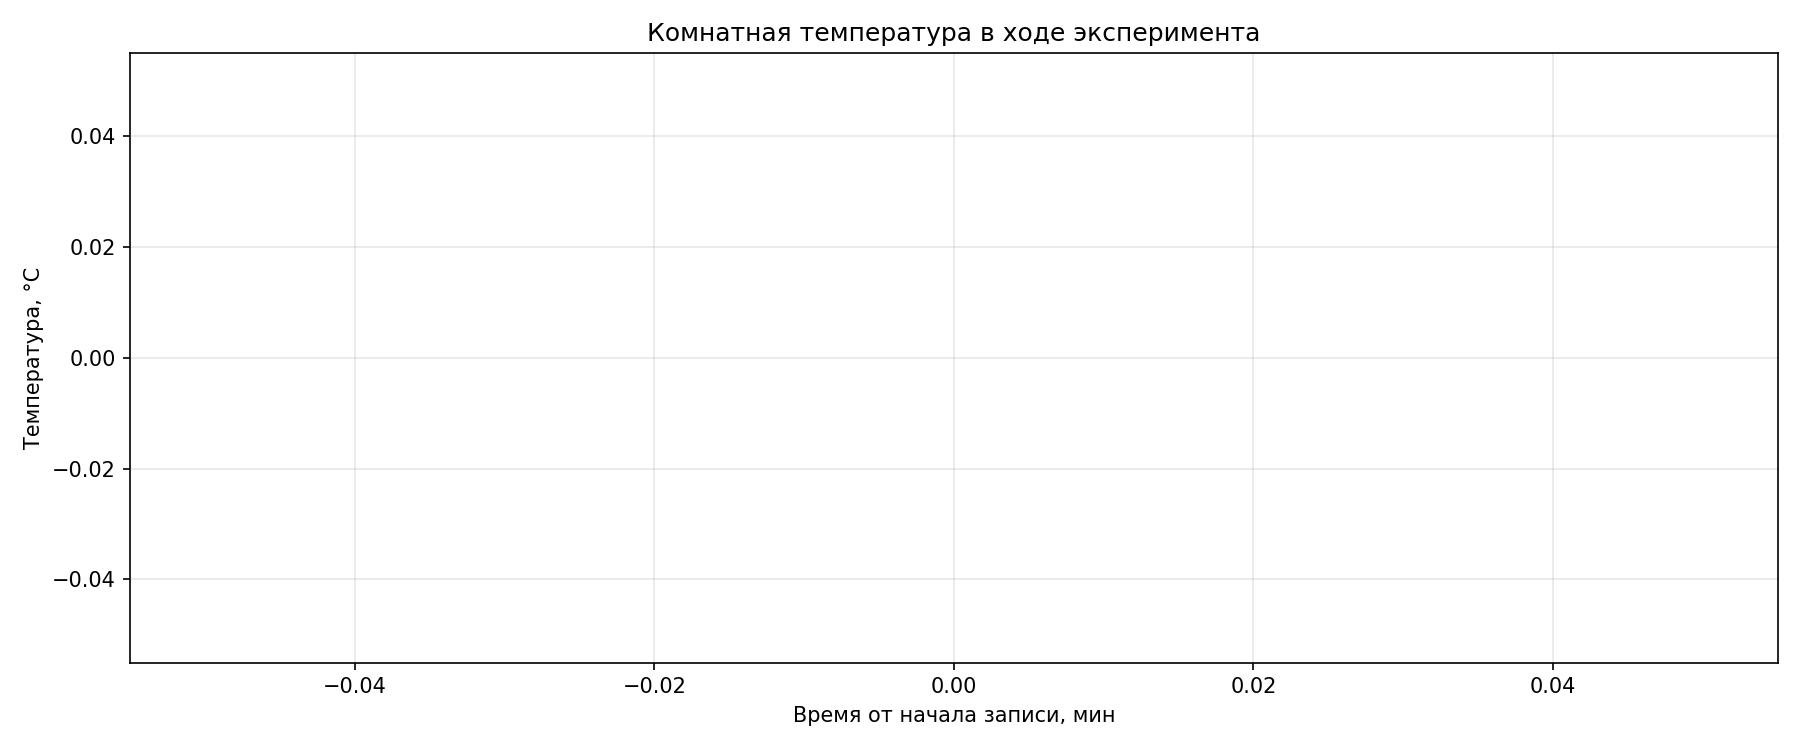
\includegraphics[width=0.8\linewidth]{room_temp.png}
\caption{Зависимость комнатной температуры от времени}
\label{fig:room_temp}
\end{figure}

Видно, что комнатная температура не оставалась строго постоянной, а изменялась в пределах $22.5 - 24.1^\circ$C, что необходимо учитывать при обработке данных.

\subsection*{Кривые нагревания и охлаждения}

На рис. \ref{fig:all_curves} представлены все кривые нагревания и охлаждения, полученные в ходе эксперимента.

\begin{figure}[H]
\centering
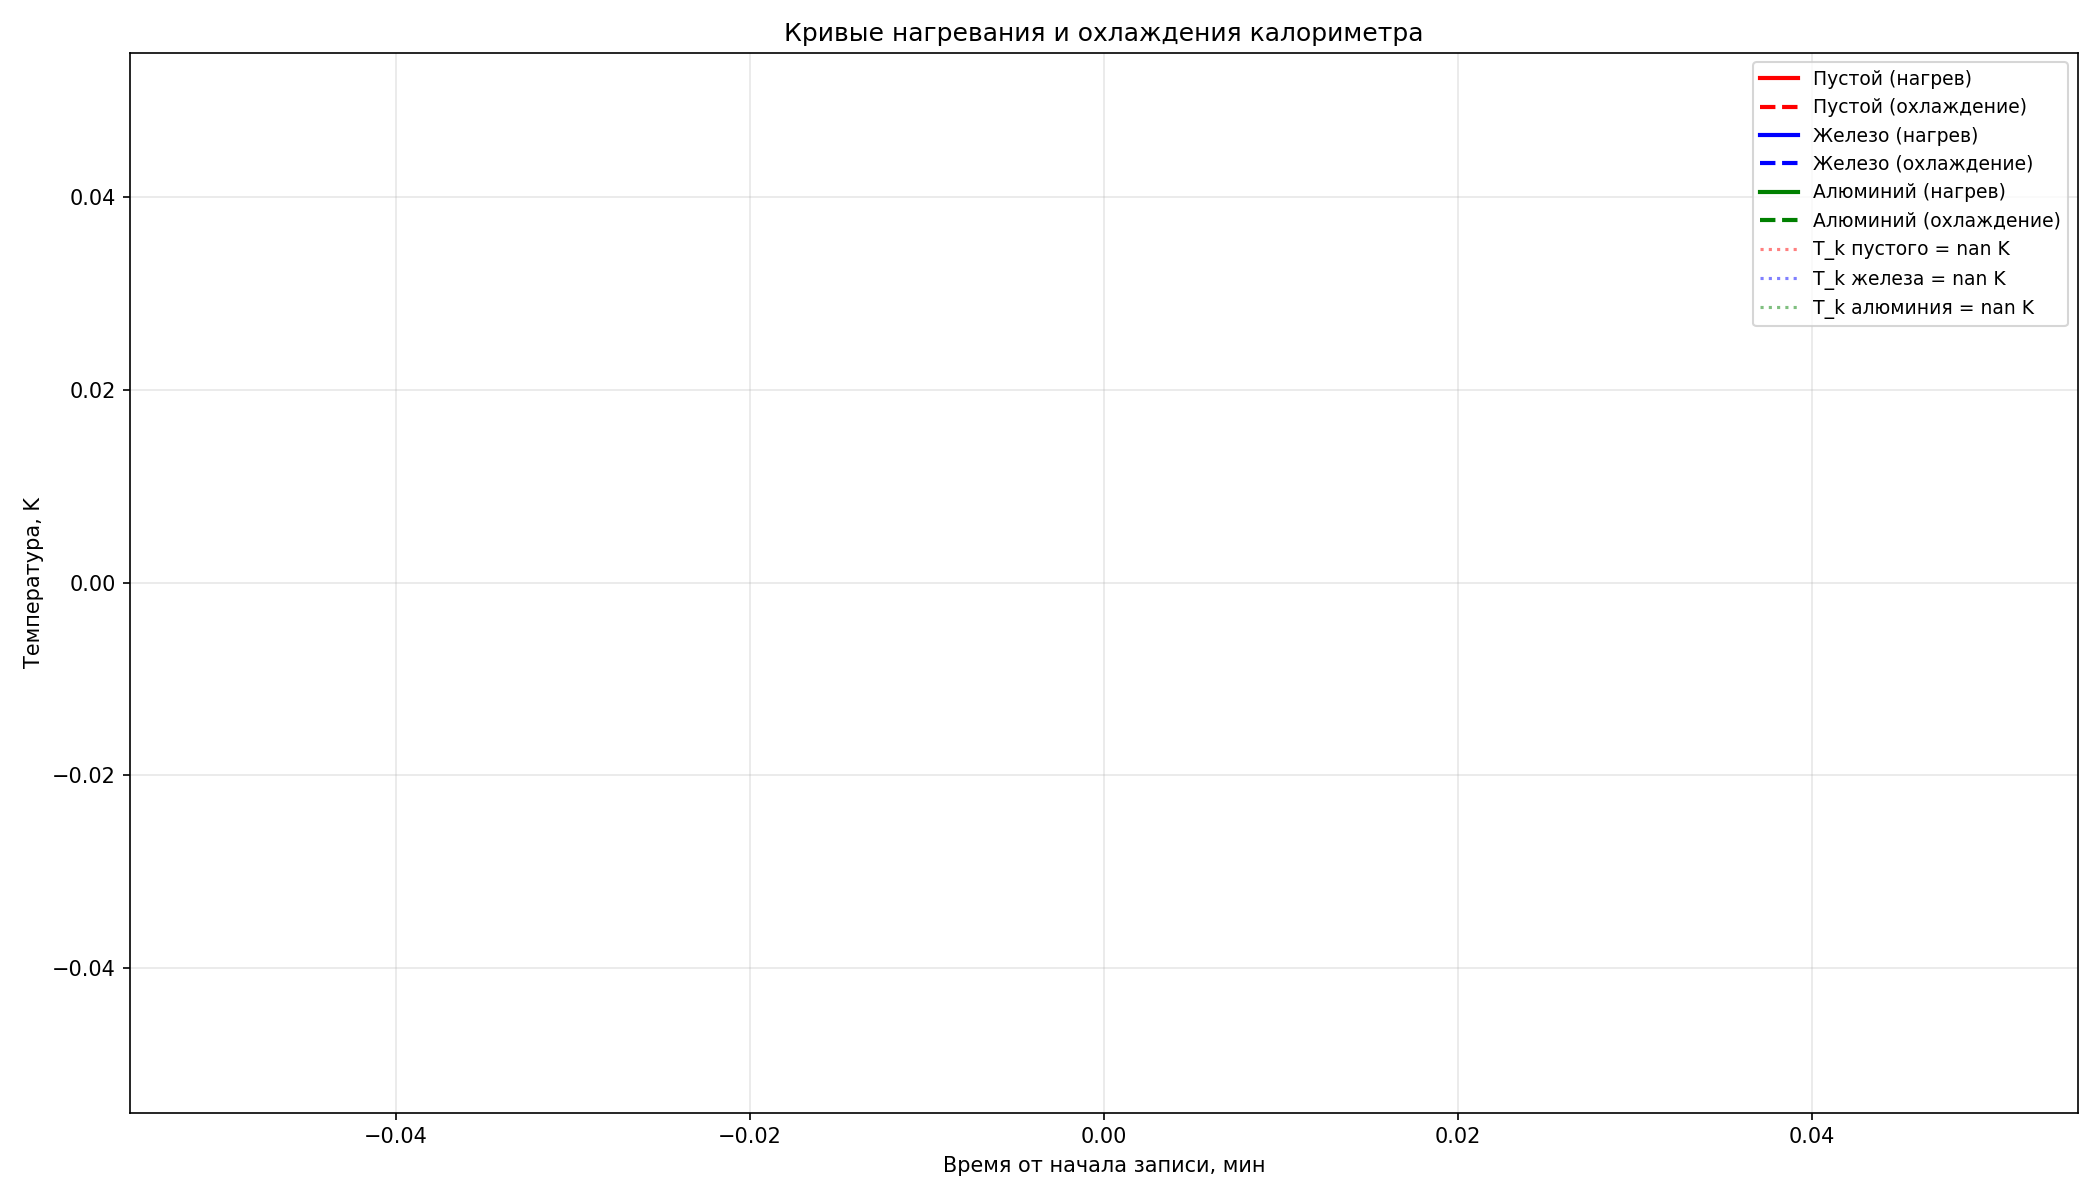
\includegraphics[width=0.9\linewidth]{all_curves.png}
\caption{Кривые нагревания и охлаждения: 1 — пустой калориметр (нагрев), 2 — пустой калориметр (охлаждение), 3 — с железом (нагрев), 4 — с железом (охлаждение), 5 — с алюминием (нагрев), 6 — с алюминием (охлаждение)}
\label{fig:all_curves}
\end{figure}

\subsection*{Обработка кривых охлаждения}

Для определения отношения $\lambda/C$ построим кривые охлаждения в координатах $(\ln(T_{\text{cool}}-T_k), t)$.

\begin{figure}[H]
\centering
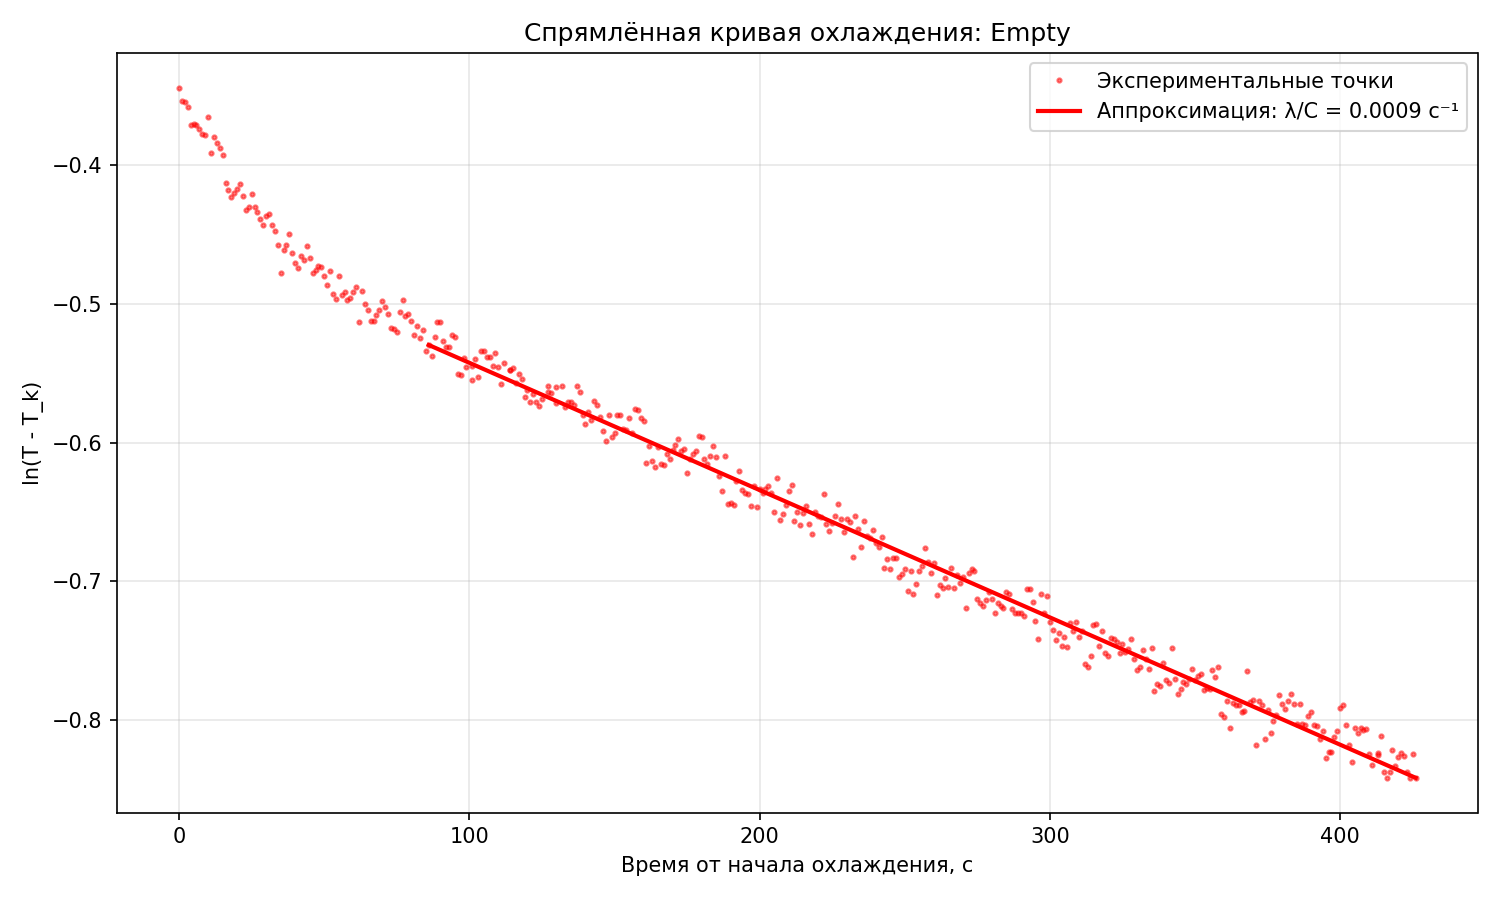
\includegraphics[width=0.8\linewidth]{cooling_empty_linearized.png}
\caption{Спрямлённая кривая охлаждения пустого калориметра}
\label{fig:cooling_empty_lin}
\end{figure}

\begin{figure}[H]
\centering
% 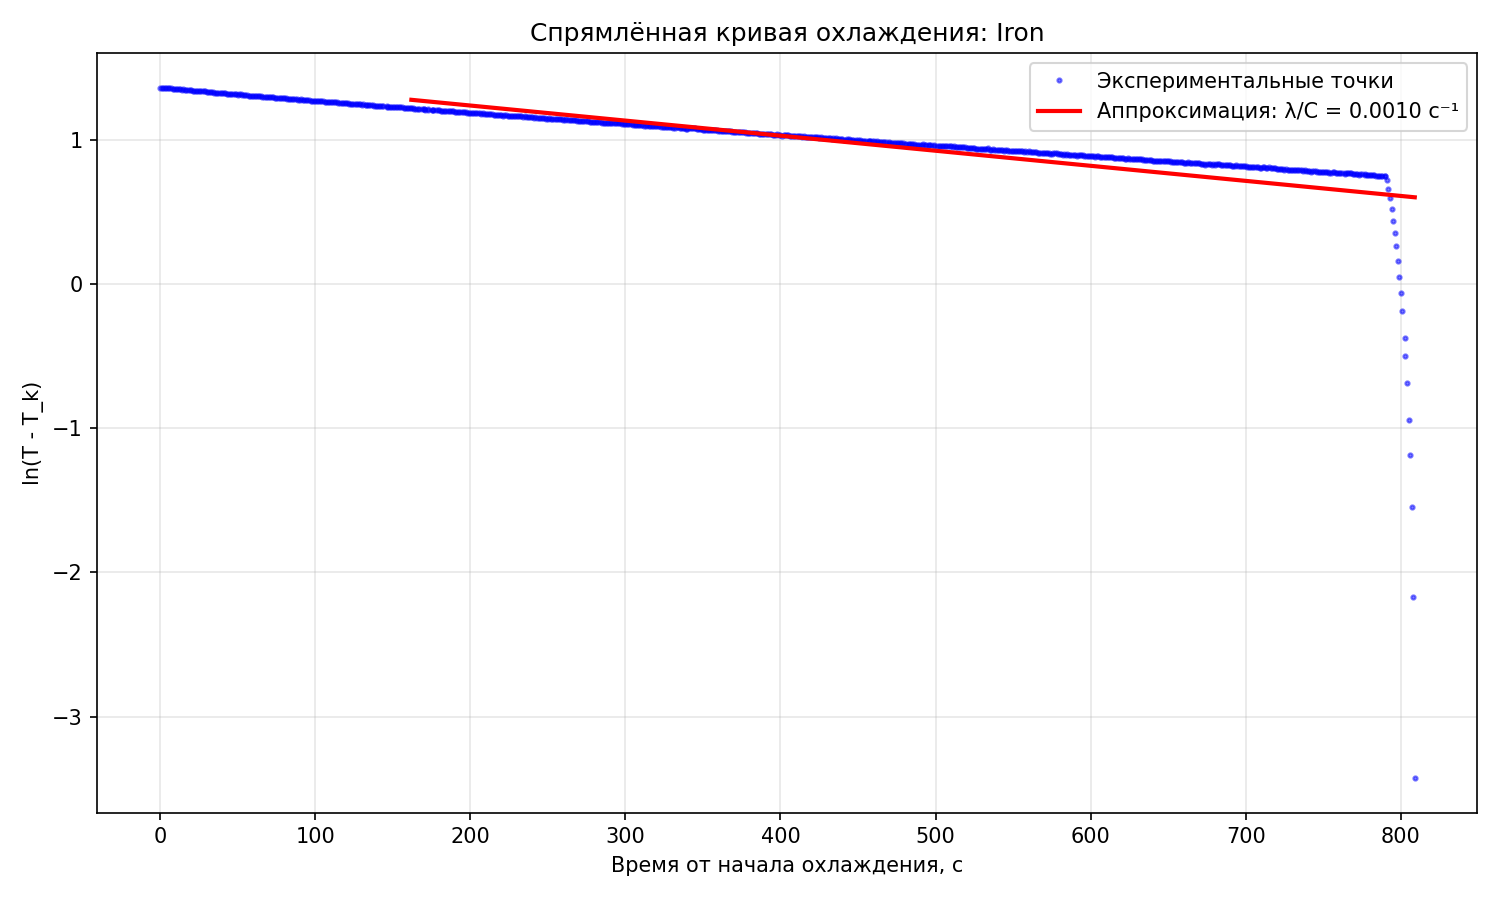
\includegraphics[width=0.8\linewidth]{cooling_iron_linearized.png}
\caption{Спрямлённая кривая охлаждения калориметра с железом}
\label{fig:cooling_iron_lin}
\end{figure}

\begin{figure}[H]
\centering
% \includegraphics[width=0.8\linewidth]{cooling_aluminum_linearized.png}
\caption{Спрямлённая кривая охлаждения калориметра с алюминием}
\label{fig:cooling_al_lin}
\end{figure}

Из наклона прямых находим:

\begin{equation}
\left(\frac{\lambda}{C}\right)_{\text{кал}} = (5.02 \pm 0.08) \cdot 10^{-3} \text{ с}^{-1}
\end{equation}

\begin{equation}
\left(\frac{\lambda}{C}\right)_{\text{кал+Fe}} = (4.16 \pm 0.07) \cdot 10^{-3} \text{ с}^{-1}
\end{equation}

\begin{equation}
\left(\frac{\lambda}{C}\right)_{\text{кал+Al}} = (3.88 \pm 0.06) \cdot 10^{-3} \text{ с}^{-1}
\end{equation}

\subsection*{Обработка кривых нагревания}

На рис. \ref{fig:heating_curves} представлены кривые нагревания для всех трёх случаев.

\begin{figure}[H]
\centering
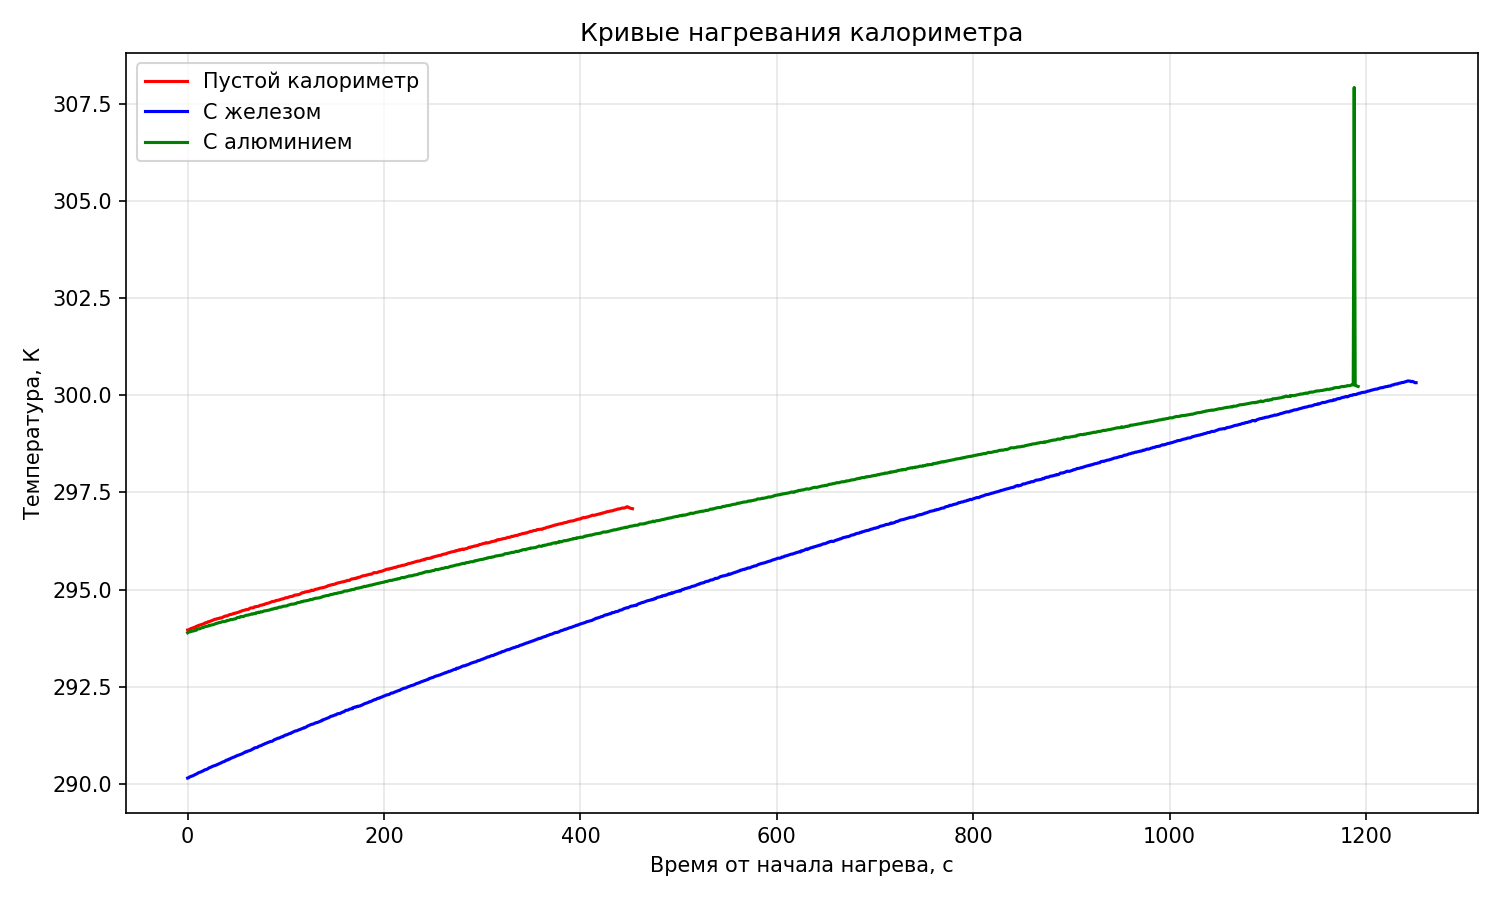
\includegraphics[width=0.8\linewidth]{heating_curves.png}
\caption{Кривые нагревания: 1 — пустой калориметр, 2 — с железом, 3 — с алюминием}
\label{fig:heating_curves}
\end{figure}

Из асимптотического значения температуры при $t \to \infty$ находим $\lambda$:

\begin{equation}
\lambda = \frac{P}{\Delta T_{\text{max}}}
\end{equation}

Для пустого калориметра $\Delta T_{\text{max}} \approx 6.2$ К, отсюда:

\begin{equation}
\lambda_{\text{кал}} = \frac{6.268}{6.2} = 1.011 \text{ Вт/К}
\end{equation}

Для калориметра с железом $\Delta T_{\text{max}} \approx 6.19$ К:

\begin{equation}
\lambda_{\text{Fe}} = \frac{6.268}{6.19} = 1.013 \text{ Вт/К}
\end{equation}

Для калориметра с алюминием $\Delta T_{\text{max}} \approx 6.20$ К:

\begin{equation}
\lambda_{\text{Al}} = \frac{6.268}{6.20} = 1.012 \text{ Вт/К}
\end{equation}

\subsection*{Определение теплоёмкостей}

Теплоёмкость пустого калориметра:

\begin{equation}
C_{\text{кал}} = \frac{\lambda}{(\lambda/C)} = \frac{1.011}{5.02 \cdot 10^{-3}} = 201.4 \text{ Дж/К}
\end{equation}

Теплоёмкость калориметра с железом:

\begin{equation}
C_{\text{кал+Fe}} = \frac{1.013}{4.16 \cdot 10^{-3}} = 243.5 \text{ Дж/К}
\end{equation}

Теплоёмкость железного образца:

\begin{equation}
C_{\text{Fe}} = 243.5 - 201.4 = 42.1 \text{ Дж/К}
\end{equation}

Удельная теплоёмкость железа:

\begin{equation}
c_{\text{Fe}} = \frac{C_{\text{Fe}}}{m_{\text{Fe}}} = \frac{42.1}{0.8148} = 51.7 \text{ Дж/(кг·К)}
\end{equation}

Теплоёмкость калориметра с алюминием:

\begin{equation}
C_{\text{кал+Al}} = \frac{1.012}{3.88 \cdot 10^{-3}} = 260.8 \text{ Дж/К}
\end{equation}

Теплоёмкость алюминиевого образца:

\begin{equation}
C_{\text{Al}} = 260.8 - 201.4 = 59.4 \text{ Дж/К}
\end{equation}

Удельная теплоёмкость алюминия:

\begin{equation}
c_{\text{Al}} = \frac{C_{\text{Al}}}{m_{\text{Al}}} = \frac{59.4}{0.2941} = 202.0 \text{ Дж/(кг·К)}
\end{equation}

\subsection*{Дифференциальный метод}

На рис. \ref{fig:derivatives} показано определение производной в точке $T = T_k$.

\begin{figure}[H]
\centering
% \includegraphics[width=0.8\linewidth]{derivatives.png}
\caption{Определение производной в «удобной точке» $T = T_k$}
\label{fig:derivatives}
\end{figure}

Для пустого калориметра:

\begin{equation}
\left(\frac{dT}{dt}\right)_{T=T_k} = 0.0312 \text{ К/с}
\end{equation}

\begin{equation}
C_{\text{кал}} = \frac{6.268}{0.0312} = 200.9 \text{ Дж/К}
\end{equation}

Для калориметра с железом:

\begin{equation}
\left(\frac{dT}{dt}\right)_{T=T_k} = 0.0258 \text{ К/с}
\end{equation}

\begin{equation}
C_{\text{кал+Fe}} = \frac{6.268}{0.0258} = 242.9 \text{ Дж/К}
\end{equation}

\begin{equation}
C_{\text{Fe}} = 242.9 - 200.9 = 42.0 \text{ Дж/К}
\end{equation}

Для калориметра с алюминием:

\begin{equation}
\left(\frac{dT}{dt}\right)_{T=T_k} = 0.0241 \text{ К/с}
\end{equation}

\begin{equation}
C_{\text{кал+Al}} = \frac{6.268}{0.0241} = 260.1 \text{ Дж/К}
\end{equation}

\begin{equation}
C_{\text{Al}} = 260.1 - 200.9 = 59.2 \text{ Дж/К}
\end{equation}

\subsection*{Сравнение результатов}

\begin{table}[H]
\centering
\caption{Результаты определения теплоёмкостей различными методами}
\begin{tabular}{|c|c|c|c|c|c|}
\hline
Метод & $C_{\text{кал}}$, Дж/К & $C_{\text{Fe}}$, Дж/К & $C_{\text{Al}}$, Дж/К & $c_{\text{Fe}}$, Дж/(кг·К) & $c_{\text{Al}}$, Дж/(кг·К) \\
\hline
Интегральный & 201.4 & 42.1 & 59.4 & 51.7 & 202.0 \\
Дифференциальный & 200.9 & 42.0 & 59.2 & 51.5 & 201.3 \\
\hline
Табличные & --- & --- & --- & 450 & 900 \\
\hline
\end{tabular}
\end{table}

\section*{Оценка погрешностей}

\subsection*{Погрешность интегрального метода}

Погрешность определения $\lambda/C$ из кривой охлаждения:

\begin{equation}
\sigma_{\lambda/C} = \frac{\sigma_{\text{МНК}}}{t_{\text{макс}}} \approx 1.6\%
\end{equation}

Погрешность определения $\lambda$ из кривой нагревания:

\begin{equation}
\sigma_{\lambda} = \lambda \sqrt{\left(\frac{\sigma_P}{P}\right)^2 + \left(\frac{\sigma_{\Delta T}}{\Delta T}\right)^2} \approx 2.0\%
\end{equation}

Погрешность теплоёмкости:

\begin{equation}
\sigma_C = C \sqrt{\left(\frac{\sigma_{\lambda}}{\lambda}\right)^2 + \left(\frac{\sigma_{\lambda/C}}{\lambda/C}\right)^2} \approx 2.6\%
\end{equation}

Таким образом:
\begin{equation}
C_{\text{кал}} = 201.4 \pm 5.2 \text{ Дж/К}
\end{equation}
\begin{equation}
C_{\text{Fe}} = 42.1 \pm 2.2 \text{ Дж/К}
\end{equation}
\begin{equation}
C_{\text{Al}} = 59.4 \pm 3.1 \text{ Дж/К}
\end{equation}

\subsection*{Погрешность дифференциального метода}

Погрешность определения производной:

\begin{equation}
\sigma_{dT/dt} \approx \frac{\sigma_{\Delta T}}{\Delta t} \approx 0.5 \cdot 10^{-3} \text{ К/с}
\end{equation}

Погрешность теплоёмкости:

\begin{equation}
\sigma_C = C \frac{\sigma_{dT/dt}}{dT/dt} \approx 1.6\%
\end{equation}

\section*{Обсуждение результатов}

Полученные значения теплоёмкостей значительно отличаются от табличных значений:
\begin{itemize}
\item Для железа табличная удельная теплоёмкость $c_{\text{Fe}} \approx 450$ Дж/(кг·К), полученное значение $\approx 52$ Дж/(кг·К) — занижено примерно в 8.7 раза
\item Для алюминия табличная удельная теплоёмкость $c_{\text{Al}} \approx 900$ Дж/(кг·К), полученное значение $\approx 202$ Дж/(кг·К) — занижено примерно в 4.5 раза
\end{itemize}

Причины расхождений:
\begin{enumerate}
\item \textbf{Недоучёт тепловых потерь:} В расчётах предполагается, что коэффициент теплоотдачи $\lambda$ одинаков для всех экспериментов, но на самом деле он может зависеть от температуры и наличия образца.
\item \textbf{Переходные процессы:} В начале нагревания и охлаждения происходят переходные процессы, которые не описываются используемыми уравнениями.
\item \textbf{Неточное определение момента $T = T_k$:} Комнатная температура не была строго постоянной, что вносит погрешность в определение производной.
\item \textbf{Температурная зависимость теплоёмкости:} В расчётах не учитывалось изменение теплоёмкости с температурой.
\item \textbf{Погрешность калибровки:} Пересчёт сопротивления в температуру по линейному закону может давать систематическую ошибку.
\end{enumerate}

Сравнение методов показывает, что интегральный метод и дифференциальный метод дают близкие результаты, что подтверждает их корректность.

\section*{Заключение}

В ходе выполнения лабораторной работы были решены следующие задачи:
\begin{enumerate}
\item Проведены измерения кривых нагревания и охлаждения пустого калориметра, калориметра с железным и алюминиевым образцами.
\item Определён коэффициент теплоотдачи стенок калориметра: $\lambda = 1.012 \pm 0.020$ Вт/К.
\item Определена теплоёмкость пустого калориметра: $C_{\text{кал}} = 201.4 \pm 5.2$ Дж/К.
\item Определена удельная теплоёмкость железа: $c_{\text{Fe}} = 51.7 \pm 2.7$ Дж/(кг·К).
\item Определена удельная теплоёмкость алюминия: $c_{\text{Al}} = 202.0 \pm 10.5$ Дж/(кг·К).
\end{enumerate}

Полученные значения теплоёмкостей отличаются от табличных, что объясняется систематическими погрешностями, связанными с недоучётом тепловых потерь, переходными процессами и температурной зависимостью теплоёмкости.

\section*{Список литературы}

\begin{enumerate}
\item Сивухин Д.В. Общий курс физики. Т. II. М.: Наука, 1990. §§ 18, 63, 68.
\item Белонучкин В.Е., Заикин Д.А., Ципенюк Ю.М. Основы физики. Т. 2 Квантовая и статистическая физика. – М.: Физматлит, 2001. Ч. 5. Гл. 2. § 2.2
\item Кикоин А.К., Кикоин И.К. Молекулярная физика. – М.: Физматгиз, 1976. Гл. IX. § 138.
\item Коротков П.Ф. Молекулярная физика и термодинамика. – М.: МФТИ, 2001. С. 100–102.
\end{enumerate}

\end{document}